% =====================================================================
% Learning to Push a T Block Through a Learned World Model
% SuperMimic style training compared with PPO on the Push-T task
%
% Compiler: pdfLaTeX. Compile twice so the contents and references update.
% Figures live in figures/. Missing images appear as labelled placeholders.
% =====================================================================

\documentclass[11pt,a4paper]{article}

% ---------------------------------------------------------------------
% Packages
% ---------------------------------------------------------------------
\usepackage[utf8]{inputenc}
\usepackage[T1]{fontenc}
\usepackage[english]{babel}
\IfFileExists{lmodern.sty}{\usepackage{lmodern}}{}
\usepackage{microtype}
\usepackage[a4paper,left=2.4cm,right=2.4cm,top=2.6cm,bottom=2.6cm,headheight=15pt]{geometry}
\usepackage{graphicx}
\usepackage[table]{xcolor}
\usepackage{array}
\usepackage{tabularx}
\usepackage{booktabs}
\usepackage{amsmath}
\usepackage{amssymb}
\usepackage{enumitem}
\usepackage{caption}
\usepackage{fancyhdr}
\usepackage{titlesec}
\usepackage[most]{tcolorbox}
\usepackage[section]{placeins}
\usepackage{listings}
\usepackage{tikz}
\usetikzlibrary{arrows.meta,positioning}
\usepackage{xurl}
\usepackage{hyperref}

% ---------------------------------------------------------------------
% Colours: ink, greys and one quiet accent
% ---------------------------------------------------------------------
\definecolor{Ink}{HTML}{1C1C1C}
\definecolor{Body}{HTML}{262626}
\definecolor{Muted}{HTML}{6A6A6A}
\definecolor{Rule}{HTML}{B5B5B5}
\definecolor{Paper}{HTML}{F5F5F3}
\definecolor{Accent}{HTML}{3B3F45}

\color{Body}
\setlength{\parindent}{0pt}
\setlength{\parskip}{6pt}
\linespread{1.07}
\setlength{\emergencystretch}{2em}
\hyphenpenalty=2000
\exhyphenpenalty=2000
\setcounter{tocdepth}{1}

\setlist[itemize]{leftmargin=1.5em,itemsep=3pt,topsep=4pt,parsep=0pt}
\setlist[enumerate]{leftmargin=1.7em,itemsep=4pt,topsep=4pt,parsep=0pt}

\hypersetup{
  colorlinks=true, linkcolor=Ink, urlcolor=Accent, citecolor=Ink,
  pdftitle={Learning to Push a T Block Through a Learned World Model},
  pdfauthor={Abyead Zarif Hassan},
  pdfsubject={Research implementation report}
}
\urlstyle{same}

% ---------------------------------------------------------------------
% Headings
% ---------------------------------------------------------------------
\titleformat{\section}{\Large\bfseries\color{Ink}}{\thesection}{0.7em}{}[\vspace{2pt}{\color{Rule}\titlerule}]
\titleformat{\subsection}{\large\bfseries\color{Ink}}{\thesubsection}{0.6em}{}
\titleformat{\subsubsection}{\normalsize\bfseries\itshape\color{Ink}}{\thesubsubsection}{0.6em}{}
\titlespacing*{\section}{0pt}{20pt}{9pt}
\titlespacing*{\subsection}{0pt}{13pt}{5pt}
\titlespacing*{\subsubsection}{0pt}{10pt}{4pt}

% ---------------------------------------------------------------------
% Header and footer
% ---------------------------------------------------------------------
\pagestyle{fancy}
\fancyhf{}
\fancyhead[L]{\small\color{Muted}Learning to push a T block through a learned world model}
\fancyhead[R]{\small\color{Muted}Abyead Zarif Hassan}
\fancyfoot[L]{\small\color{Muted}Research implementation report}
\fancyfoot[R]{\small\color{Ink}\thepage}
\renewcommand{\headrulewidth}{0.4pt}
\renewcommand{\headrule}{{\color{Rule}\hrule width\headwidth height\headrulewidth}}
\renewcommand{\footrulewidth}{0pt}

% ---------------------------------------------------------------------
% Captions and tables
% ---------------------------------------------------------------------
\captionsetup{font=small,labelfont={bf,color=Ink},justification=justified,singlelinecheck=false,skip=7pt}
\captionsetup[table]{position=top}
\newcolumntype{L}{>{\raggedright\arraybackslash}X}
\newcolumntype{C}{>{\centering\arraybackslash}X}
\arrayrulecolor{Rule}
\setlength{\tabcolsep}{5pt}
\renewcommand{\arraystretch}{1.28}
\newcommand{\thd}[1]{\textbf{\color{Ink}#1}}

% ---------------------------------------------------------------------
% Boxes: a thin grey rule on the left, no colour fill beyond paper grey
% ---------------------------------------------------------------------
\tcbset{
  reportbox/.style={enhanced,breakable,frame hidden,boxrule=0pt,sharp corners,
    colback=Paper,borderline west={1.6pt}{0pt}{Accent},
    left=11pt,right=10pt,top=7pt,bottom=7pt,before skip=9pt,after skip=9pt,
    fonttitle=\bfseries\small,coltitle=Ink,colbacktitle=Paper,titlerule=0pt,
    attach title to upper={\par\smallskip}}
}
\newtcolorbox{summarybox}[1][Main observation]{reportbox,title={#1}}
\newtcolorbox{notebox}[1][Interpretation]{reportbox,title={#1}}
\newtcolorbox{limitbox}[1][Limitation]{reportbox,borderline west={1.6pt}{0pt}{Muted},title={#1}}

% ---------------------------------------------------------------------
% Code
% ---------------------------------------------------------------------
\lstset{basicstyle=\ttfamily\footnotesize,backgroundcolor=\color{Paper},frame=single,
  rulecolor=\color{Rule},framerule=0.4pt,breaklines=true,columns=fullflexible,keepspaces=true,
  showstringspaces=false,xleftmargin=5pt,xrightmargin=5pt,framexleftmargin=5pt,
  framexrightmargin=5pt,aboveskip=9pt,belowskip=9pt}

% ---------------------------------------------------------------------
% Figures with a placeholder when the file is missing
% ---------------------------------------------------------------------
\newcommand{\reportfigure}[4][0.96]{
  \begin{figure}[htbp]
    \centering
    \IfFileExists{#2}{\includegraphics[width=#1\linewidth,height=0.42\textheight,keepaspectratio]{#2}}{
      \begin{tcolorbox}[width=0.9\linewidth,colback=Paper,colframe=Rule,boxrule=0.5pt,sharp corners]
        \centering\vspace{10pt}\textbf{Figure file not found}\\[4pt]\texttt{\detokenize{#2}}\\[4pt]
        Run \texttt{python report/make\_figures.py} from the repository root.\vspace{10pt}
      \end{tcolorbox}}
    \caption{#3}
    \label{#4}
  \end{figure}
}

\renewcommand{\cite}[1]{\ref{ref:#1}}
\newcommand{\repo}{\url{https://github.com/AbyeadZarifHassan/pusht-supermimic}}

% =====================================================================
\begin{document}
% =====================================================================

% ---------------------------------------------------------------------
% Title page
% ---------------------------------------------------------------------
\begin{titlepage}
\thispagestyle{empty}
\begingroup
\setlength{\parskip}{4pt}
\setlength{\parindent}{0pt}

{\color{Ink}\hrule height 1.2pt}
\vspace{0.18cm}
{\small\color{Muted}\textsc{Research Implementation Report}\hfill\textsc{University of Dhaka}\par}
\vspace{1.5cm}

{\fontsize{26}{32}\selectfont\bfseries\color{Ink}
Learning to Push a T Block\\
Through a Learned\\
World Model\par}

\vspace{0.5cm}
{\large\itshape\color{Muted}
SuperMimic style backpropagation through time\\
compared with PPO on the Push-T manipulation task\par}

\vspace{0.6cm}
{\color{Rule}\hrule height 0.5pt}
\vspace{0.55cm}

\begin{minipage}[t]{0.47\textwidth}
  {\small\color{Muted}\textsc{Author}\par}
  \vspace{2pt}
  {\large\bfseries\color{Ink}Abyead Zarif Hassan\par}
  {\normalsize BSc in Robotics and Mechatronics Engineering\\University of Dhaka\par}
\end{minipage}\hfill
\begin{minipage}[t]{0.47\textwidth}
  {\small\color{Muted}\textsc{Prepared for}\par}
  \vspace{2pt}
  {\large\bfseries\color{Ink}Dr Chengzhou Tang\par}
  {\normalsize Spatial Intelligent System Lab\\University of Manitoba\par}
\end{minipage}

\vspace{0.9cm}

\begin{tcolorbox}[reportbox,breakable=false,title={Report overview},fontupper=\small,before skip=0pt,after skip=0pt]
Dr Tang's case study on SuperMimic ends with an open question: does training a policy through a
learned differentiable world model still work when the reward is sparse and the task is
manipulation without a reference trajectory? I tested this on Push-T. I built the simulator, a
SuperMimic style learner and a PPO baseline, and ran both under the same observation and action
design.

\smallskip
With a shaped reward and a 16 step imagination horizon the SuperMimic style learner solved
\textbf{87\% of 100 unseen episodes} from the original Push-T start distribution. PPO stayed at 0\%
with the same data budget. With a purely sparse reward both methods failed completely.

\smallskip
The results come from one or two random seeds on a desktop CPU. Training was also unstable even in
the best run. I treat the numbers as evidence about this setup rather than as a general ranking of
the two methods.
\end{tcolorbox}

\vfill
\noindent\begin{minipage}{\textwidth}
  {\color{Rule}\hrule height 0.5pt}
  \vspace{0.2cm}
  {\small\color{Muted}November 2026\hfill Based on the case study \emph{SuperMimic} by Dr Chengzhou Tang\par
  \vspace{2pt}
  Code and results: \repo\par}
\end{minipage}
\endgroup
\end{titlepage}

% ---------------------------------------------------------------------
\pagenumbering{roman}
\tableofcontents
\clearpage
\pagenumbering{arabic}

% =====================================================================
\section{Purpose of the work}
\label{sec:purpose}

Dr Tang gave me three sets of material: two lectures on reinforcement learning and a case study
of the SuperMimic paper~\cite{supermimic}. The task was to read them and implement the ideas on
the Push-T task. I also had the paper by Ma et al.~\cite{esm} which uses Push-T as its benchmark
for training policies with reinforcement learning from a sparse reward.

SuperMimic trains a humanoid to track human motion. Its key idea is to learn a neural network that
imitates the physics simulator and then train the policy by sending gradients through that network
over a short imagined rollout. The case study closes with a list of open questions. The first one
is the one this report tries to answer:

\begin{notebox}[The question from the case study]
\emph{Sparse rewards? Manipulation and locomotion without a reference trajectory.}

Motion tracking gives a dense reward at every step because a reference motion says where every joint
should be. Push-T is the opposite. The natural reward is 1 only when the T block covers 95\% of a
goal outline and 0 otherwise. Contact between the pusher and the block also decides everything.
\end{notebox}

I made four questions out of this and designed the experiments around them:
\begin{enumerate}
  \item Does a SuperMimic style learner beat a likelihood ratio method such as PPO on Push-T with
        the same amount of data?
  \item Does it still work when the reward is purely sparse?
  \item Does the critic matter when the imagination horizon is short?
  \item Are gradients through contact smooth enough for backpropagation through time? The case study
        lists this as an assumption.
\end{enumerate}

% =====================================================================
\section{Background}
\label{sec:background}

\subsection{Two ways to estimate a policy gradient}

The lectures present two families of policy gradient estimators. I use their names throughout.

\textbf{Likelihood ratio.} REINFORCE~\cite{reinforce} and PPO~\cite{ppo} never differentiate
the environment. They raise the log probability of actions that turned out better than expected:
\begin{equation}
  \nabla_\theta J \approx \mathbb{E}\big[\nabla_\theta \log \pi_\theta(a_t \mid s_t)\, \hat{A}_t\big].
\end{equation}
The simulator can be a black box. The price is variance. Baselines, advantages and
GAE~\cite{gae} exist mainly to reduce it, and PPO needs fresh data after every update because it
is on policy.

\textbf{Pathwise.} If the dynamics $s_{t+1}=f(s_t,a_t)$ and the reward are differentiable, the
return of a rollout can be differentiated with respect to the policy parameters directly:
\begin{equation}
  \nabla_\theta J = \nabla_\theta \sum_{t=0}^{H-1} \gamma^t\, r\big(s_t, \pi_\theta(s_t)\big),
  \qquad s_{t+1} = f\big(s_t,\pi_\theta(s_t)\big).
\end{equation}
Every action gets an exact gradient, so the variance is low. The catch is that $f$ must be
differentiable and its gradients must be useful. Through contact they can be large or
discontinuous~\cite{suh}.

\subsection{SuperMimic}

SuperMimic~\cite{supermimic} does not differentiate the simulator. It learns a world model
$f_\omega$ from logged transitions and differentiates that instead. Training repeats three steps:
collect data with the current policy, fit the world model, then improve the policy by
backpropagation through time (BPTT) over imagined rollouts of the frozen model. A critic estimates
the value after the last imagined step so that the horizon can stay short. Because physics does not
depend on which policy collected the data, old transitions remain useful and the method is off
policy. The paper reports more than a thousand times fewer GPU hours than PPO for humanoid
motion tracking.

\subsection{Push-T}

Push-T~\cite{diffpolicy} is a planar task. A circular pusher moves on a $512 \times 512$ pixel
table and must push a T shaped block onto a fixed goal pose. An episode succeeds when the block
covers at least 95\% of the goal area. Ma et al.~\cite{esm} train policies on it with online
reinforcement learning from a sparse reward. They report that PPO and SAC with Gaussian policies
struggle, and they rely on two design choices that I copied: an observation expressed in the frame
of the block and a reverse curriculum that starts the block close to the goal.

% =====================================================================
\section{The Push-T environment}
\label{sec:env}

I wrote my own simulator in \texttt{pusht\_rl/env.py} using the pymunk physics engine. It follows
the geometry and rates of the original Push-T task and does not need pygame or MuJoCo. It runs on
Linux and on Windows.

\begin{table}[htbp]
\centering
\small
\caption{Environment settings.}
\label{tab:env}
\begin{tabularx}{\textwidth}{p{4.2cm}L}
\toprule
\thd{Setting} & \thd{Value} \\
\midrule
Table and objects & $512\times512$ px table, pusher radius 15 px, T made of a $120\times30$ px bar and a $30\times90$ px stem \\
Goal pose & $(256, 256)$ px and $\pi/4$ rad, fixed \\
Physics and control rate & 100 Hz physics, 10 Hz control \\
Action & Pusher velocity in the goal frame, $a \in [-1,1]^2$, scaled to 200 px/s \\
Observation & Pusher and goal position in the block frame, $\sin$ and $\cos$ of the goal angle in the block frame, block velocity in the block frame (9 numbers) \\
Success & At least 95\% of the goal area covered \\
Episode limit & 300 control steps \\
Table friction & The block loses 99\% of its velocity per second (see Section~\ref{sec:friction}) \\
Reverse curriculum & Stage $m$ starts the block within $256 \pm (30 + 100\,m/10)$ px; the stage advances after 50 successes \\
\bottomrule
\end{tabularx}
\end{table}

\reportfigure[0.92]{figures/task.pdf}
{The task. The dashed outline is the goal pose and the grey shapes are example starting poses.
At curriculum stage 0 the block starts within 30 px of the goal at any angle. By stage 10 the range
is 130 px. Evaluation always uses the original Push-T reset, where the block can start anywhere in
the dotted square at any angle.}
{fig:task}

\subsection{Rewards}

I used two reward settings.

\textbf{Sparse.} The reward is 1 on the step that reaches success and the episode ends. Every other
step gives 0. This is the setting in Ma et al.~\cite{esm} and the one the case study asks about.

\textbf{Dense.} I added potential based shaping~\cite{shaping}:
\begin{equation}
  r_t = \Phi(s_{t+1}) - \Phi(s_t) + \mathbb{1}[\text{success}],
  \qquad
  \Phi(s) = e^{-d/60}\,\tfrac{1}{2}\big(1+\cos\Delta\theta\big),
\end{equation}
where $d$ is the distance in pixels between the block and the goal and $\Delta\theta$ is the angle
between them. Shaping of this form does not change which policy is optimal. The sum of the shaping
terms over an episode telescopes, so the agent gains nothing by hovering near the goal without
finishing. I chose $\Phi$ so that the same formula can be written in PyTorch and differentiated.

% =====================================================================
\section{Method}
\label{sec:method}

\subsection{The SuperMimic style learner}

Figure~\ref{fig:loop} shows the loop. The code is in \texttt{pusht\_rl/world\_model.py} and
\texttt{pusht\_rl/supermimic.py}.

\begin{figure}[htbp]
\centering
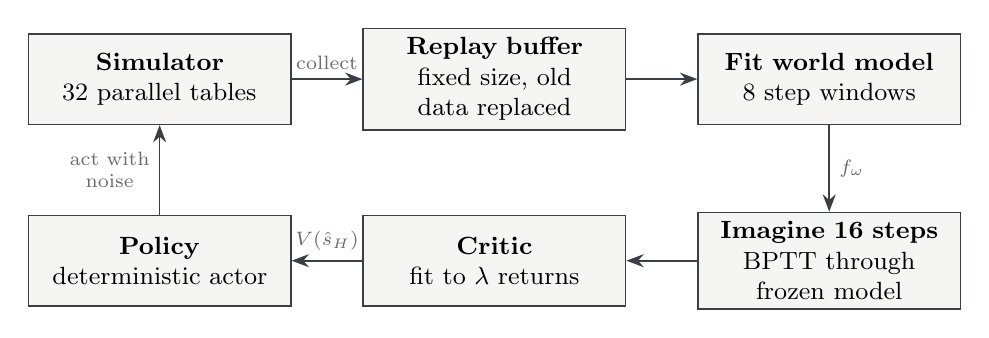
\begin{tikzpicture}[
  node distance=0.55cm and 0.9cm,
  box/.style={draw=Accent,line width=0.5pt,fill=Paper,align=center,minimum height=1.15cm,text width=3.1cm,font=\small},
  arr/.style={-{Stealth[length=2.2mm]},draw=Accent,line width=0.6pt},
  lab/.style={font=\scriptsize,color=Muted,align=center}]
\node[box] (sim) {\textbf{Simulator}\\32 parallel tables};
\node[box,right=of sim] (buf) {\textbf{Replay buffer}\\fixed size, old data replaced};
\node[box,right=of buf] (wm) {\textbf{Fit world model}\\8 step windows};
\node[box,below=1.1cm of wm] (img) {\textbf{Imagine 16 steps}\\BPTT through frozen model};
\node[box,left=of img] (crit) {\textbf{Critic}\\fit to $\lambda$ returns};
\node[box,left=of crit] (pol) {\textbf{Policy}\\deterministic actor};
\draw[arr] (sim) -- node[lab,above]{collect} (buf);
\draw[arr] (buf) -- (wm);
\draw[arr] (wm) -- node[lab,right]{$f_\omega$} (img);
\draw[arr] (img) -- (crit);
\draw[arr] (crit) -- node[lab,above]{$V(\hat s_H)$} (pol);
\draw[arr] (pol) -- node[lab,left]{act with\\noise} (sim);
\end{tikzpicture}
\caption{The training loop. Real data trains the world model. The policy is trained only on imagined
rollouts of that model, with the critic covering everything after the last imagined step.}
\label{fig:loop}
\end{figure}

\textbf{State and world model.} The model state is eight numbers: pusher position, block pose and
block linear and angular velocity. The world model is a three layer MLP with 256 units, layer
normalisation and SiLU activations. It predicts the change in pusher position and the motion of the
block. I made it predict block motion in the frame of the block and then rotate it back into the
world frame. A push from the left then looks the same wherever the block is, so the network does not
have to learn pushing again for every position and angle. It is trained on windows of $k=8$ logged
steps by rolling the model forward on its own predictions:
\begin{equation}
  \mathcal{L}_{\text{wm}} = \sum_{j=1}^{k} \big\lVert \hat s_j - s_j \big\rVert^2
  + \mathrm{BCE}\big(\hat d_j, d_j\big),
  \qquad \hat s_{j} = f_\omega(\hat s_{j-1}, a_{j-1}),\ \hat s_0 = s_0 .
\end{equation}

\textbf{Success head.} In Push-T success and termination are the same event. A small network
predicts the probability $\hat d$ that a state is a success. Successes are rare, so I train it on
batches that are half successes and then correct its output by the true success rate so that the
probability stays calibrated. The observation is computed analytically from the state and is
differentiable.

\textbf{Policy objective.} Starting from states drawn from the buffer, the actor rolls the frozen
model forward for $H$ steps. The objective is
\begin{equation}
  J(\theta) = \sum_{t=0}^{H-1} \gamma^t c_t\, \hat r_{t+1} + \gamma^H c_H\, V_\psi(\hat s_H),
  \qquad c_0 = 1,\quad c_{t+1} = c_t\,(1-\hat d_{t+1}),
\end{equation}
where $c_t$ is a soft probability that the episode is still running. For the sparse reward
$\hat r = \hat d$. For the dense reward the shaping term is added. The gradient of $J$ flows through
every model step back to the actor parameters.

\textbf{Critic.} The critic is fitted to $\lambda$ returns of the same imagined rollout, as in
SuperMimic and Dreamer~\cite{dreamer}:
\begin{equation}
  R_t^\lambda = \hat r_{t+1} + \gamma(1-\hat d_{t+1})\big[(1-\lambda)V_\psi(\hat s_{t+1}) + \lambda R_{t+1}^\lambda\big],
  \qquad R_H^\lambda = V_\psi(\hat s_H).
\end{equation}

\begin{table}[htbp]
\centering
\small
\caption{Settings of the SuperMimic style learner.}
\label{tab:sm}
\begin{tabularx}{\textwidth}{p{5.2cm}L}
\toprule
\thd{Setting} & \thd{Value} \\
\midrule
Networks & World model, actor and critic: 3 layers of 256 units with layer normalisation \\
Imagination horizon $H$ & 16 (32 and 8 in the ablations) \\
World model window $k$ & 8 steps \\
Discount $\gamma$ and $\lambda$ & 0.99 and 0.95 \\
Learning rates & World model and critic $3\times10^{-4}$, actor $1\times10^{-4}$ \\
Actor gradient clipping & Norm 0.5 \\
Batch size & 256 windows or start states \\
Updates & 4 world model updates and 4 policy updates per 256 environment steps \\
Exploration & Gaussian noise with standard deviation 0.3 on the actions \\
Replay buffer & 1 million transitions, the first 20{,}000 from random actions \\
\bottomrule
\end{tabularx}
\end{table}

\subsection{PPO baseline}

PPO~\cite{ppo} uses the same observation, action space, curriculum and simulator. The actor outputs
the mean of a Gaussian with a learned standard deviation. I used the clipped objective with
$\epsilon = 0.2$, GAE with $\gamma=0.99$ and $\lambda=0.95$, rollouts of 128 steps on 32 tables,
10 epochs per rollout, minibatches of 1024 and a learning rate of $3\times10^{-4}$. When an
episode is cut off by the time limit the value of the next state is still used, but after a
success it is not.

% =====================================================================
\section{Experimental setup}
\label{sec:setup}

All runs used an Intel Core i5-9400F with 16~GB of RAM on Windows. PPO ran its networks on an
NVIDIA RTX 4060. The SuperMimic style learner ran on the CPU because it was about 1.7 times faster
there: its networks are small and the GPU spent most of its time waiting for many tiny operations.

\textbf{Evaluation.} Every 100{,}000 environment steps the deterministic policy was tested on 100
episodes from the \emph{original} Push-T reset, not from the curriculum. I report three numbers:
\begin{itemize}
  \item \textbf{Success:} the share of episodes that reach 95\% coverage within 300 steps.
  \item \textbf{Coverage:} the mean share of the goal covered at the end of the episode. It shows
        progress long before the first success.
  \item \textbf{Episode length:} shorter means the policy finishes faster.
\end{itemize}

\textbf{A baseline that does nothing.} A policy that never moves leaves the block where it started.
It scores 0.237 coverage at curriculum stage 0 and 0.043 under the original reset. A method has only
learned something once it beats these numbers.

\textbf{Checkpoints.} The code keeps the checkpoint with the best evaluation score in a separate file
(\texttt{checkpoint\_best.pt}). Section~\ref{sec:best} reports a fresh evaluation of that checkpoint.

% =====================================================================
\section{Results}
\label{sec:results}

\subsection{Comparison after 500,000 steps}

\begin{table}[htbp]
\centering
\small
\caption{Evaluation on the original Push-T reset after 500{,}000 environment steps. Dense reward
unless stated. ``Successes in training'' counts successful training episodes so far.}
\label{tab:main}
\begin{tabularx}{\textwidth}{L>{\centering\arraybackslash}p{1.6cm}>{\centering\arraybackslash}p{1.7cm}>{\centering\arraybackslash}p{2.3cm}>{\centering\arraybackslash}p{1.6cm}}
\toprule
\thd{Method} & \thd{Success} & \thd{Coverage} & \thd{Successes in training} & \thd{Time} \\
\midrule
Do nothing & 0\% & 0.04 & -- & -- \\
PPO, sparse reward & 0\% & 0.05 & 0 & 5 min \\
PPO, dense reward & 0\% & 0.06 & 0 & 5 min \\
SuperMimic style, sparse reward, $H=16$ & 0\% & 0.05 & 0 & 38 min \\
SuperMimic style, $H=32$ & 0\% & 0.12 & 8 & 62 min \\
SuperMimic style, $H=16$, no critic & 2\% & 0.36 & -- & 28 min \\
SuperMimic style, $H=8$ & 15\% & 0.51 & 34 & 22 min \\
\textbf{SuperMimic style, $H=16$} & \textbf{15\%} & \textbf{0.55} & \textbf{61} & 35 min \\
\bottomrule
\end{tabularx}
\end{table}

\reportfigure{figures/compare_500k.pdf}
{The same comparison as Table~\ref{tab:main}. Light bars mark runs that did not beat the do nothing
policy in a meaningful way.}
{fig:compare}

With the dense reward and a short horizon the SuperMimic style learner pushes the block towards the
goal and starts to finish episodes. PPO saw the same number of steps and did not get past the do
nothing level. Its best training coverage was 0.28 at curriculum stage 0, compared with 0.237 for
doing nothing, and it never recorded a single success.

\begin{summarybox}[Main observation]
With the same 500{,}000 steps, the pathwise learner reached 15\% success and 0.55 coverage while
PPO stayed at 0\%. This matches the sample efficiency argument in the case study. PPO was about
seven times faster in wall clock time, so the comparison is about data, not about compute.
\end{summarybox}

\subsection{The long run}

I continued the $H=16$ run to two million steps. It took 2 hours and 21 minutes on the CPU.

\begin{table}[htbp]
\centering
\small
\caption{Evaluation during the two million step run (seed 0).}
\label{tab:long}
\begin{tabularx}{\textwidth}{L*{7}{C}}
\toprule
\thd{Steps} & \thd{0.5M} & \thd{1.0M} & \thd{1.2M} & \thd{1.5M} & \thd{1.7M} & \thd{1.8M} & \thd{2.0M} \\
\midrule
Curriculum stage & 1 & 5 & 9 & 10 & 10 & 10 & 10 \\
Success & 15\% & 64\% & 61\% & 85\% & \textbf{87\%} & 19\% & 79\% \\
Coverage & 0.55 & 0.81 & 0.83 & 0.88 & 0.89 & 0.50 & \textbf{0.93} \\
Episode length & 275 & 182 & 170 & 105 & \textbf{100} & 264 & 115 \\
\bottomrule
\end{tabularx}
\end{table}

\reportfigure{figures/long_run.pdf}
{Evaluation success and coverage over training. The dotted line on the right is the curriculum
stage of seed 0. A second seed is shown in grey up to the point where a power cut stopped it.}
{fig:long}

The curriculum reached its final stage at about 1.2 million steps. After that the policy kept
improving on the full Push-T distribution and its episodes became much shorter. The curve is not
smooth though. Success fell to 0\% at 700{,}000 steps, to 10\% at 1.1 million and to 19\% at 1.8
million, and recovered each time. Saving the best checkpoint separately turned out to be essential.

\subsection{Final evaluation of the best checkpoint}
\label{sec:best}

The best checkpoint came from 1.7 million steps. I evaluated it again on 100 new episodes.

\begin{table}[htbp]
\centering
\small
\caption{Fresh evaluation of the best checkpoint.}
\label{tab:best}
\begin{tabularx}{\textwidth}{LCC}
\toprule
\thd{Start distribution} & \thd{Success} & \thd{Episode length (mean $\pm$ sd)} \\
\midrule
Original Push-T reset & \textbf{87\%} & $99.8 \pm 83.1$ \\
Final curriculum range & 92\% & $87.2 \pm 70.8$ \\
\bottomrule
\end{tabularx}
\end{table}

\reportfigure{figures/rollout_frames.png}
{One evaluation episode of the best policy, from left to right. The pusher walks around the block,
turns it and slides it into the goal outline. The full animation is \texttt{docs/best\_model.gif} in
the repository.}
{fig:frames}

\subsection{The imagination horizon}

\begin{table}[htbp]
\centering
\small
\caption{Effect of the imagination horizon at 500{,}000 steps. The gradient norm is measured before
clipping.}
\label{tab:horizon}
\begin{tabularx}{\textwidth}{>{\centering\arraybackslash}p{1.8cm}CCL}
\toprule
\thd{Horizon} & \thd{Success} & \thd{Coverage} & \thd{Actor gradient norm} \\
\midrule
32 & 0\% (2\% at 200k) & 0.12 & Repeated spikes from 100 to over 3{,}000 \\
16 & 15\% & 0.55 & Mostly below 5, occasional spikes near 15 \\
8 & 15\% & 0.51 & Mostly below 1 \\
\bottomrule
\end{tabularx}
\end{table}

With $H=32$ the learner improved for 200{,}000 steps and then fell apart. Its training coverage
peaked at 0.39 and then dropped while the actor gradient norm jumped to values in the hundreds and
thousands. Halving the horizon removed most of these spikes and the run kept improving.

The gradient of $J$ with respect to an early action is a product of world model Jacobians, one for
every later step. Away from the block these Jacobians are small. When the pusher touches the block
they can be large. Multiplying thirty two of them gives a much wider range of magnitudes than
multiplying sixteen. The critic makes the shorter horizon affordable because it values everything
after the last imagined step. SuperMimic reports the same trade off for humanoids.

\subsection{The critic}

\reportfigure[0.62]{figures/ablations.pdf}
{Evaluation coverage during the first 500{,}000 steps for $H=16$ with and without a critic, and with
the sparse reward.}
{fig:ablate}

Without a critic the $H=16$ run followed the normal run closely until 400{,}000 steps and reached
11\% success there. At 500{,}000 steps it dropped to 2\% while the run with a critic rose to 15\%.
This is a single comparison, so I read it as a sign that the critic stabilises training rather than
as proof.

\subsection{Sparse reward}
\label{sec:sparse}

With the purely sparse reward the SuperMimic style learner failed completely. After one million
steps it had 0\% success, its coverage stayed between 0.05 and 0.06 and it never recorded a
successful training episode, so the curriculum never left stage 0. PPO behaved the same way. Its
value loss stayed near $10^{-8}$ because it had never seen a reward, so its advantages were
essentially noise and the policy drifted.

\begin{notebox}[Why both methods fail]
For PPO the gradient is the log probability gradient times the advantage. With no reward the
advantage is zero.

For the pathwise learner the reward in imagination is the predicted success probability. Before the
first success the success head learns that success never happens, so $\hat r$ is zero everywhere and
so is its gradient. The critic learns to predict zero as well.

Both estimators need some signal before they can follow it. Here that signal had to come from
shaping. Even in the dense runs the calibrated success head stayed around $10^{-3}$, so the success
bonus barely contributed and the shaping term did almost all the work.
\end{notebox}

\subsection{Table friction}
\label{sec:friction}

The original Push-T simulator has no friction between the block and the table, so a pushed block
keeps sliding. In my first runs I used this setting. Both learners ended up at the do nothing level.
After 150{,}000 steps the SuperMimic style learner had 0.22 coverage at stage 0 against 0.237 for
doing nothing. When I looked at its actions it had learned to keep away from the block. With a
block that keeps sliding, almost any push lowers the pose score within the imagined horizon, so not
touching the block is a local optimum of $J$.

With friction added (the block loses 99\% of its velocity per second, which is closer to a real
tabletop) the same learner reached 0.37 coverage after 150{,}000 steps and recorded its first
successes. I made this the default. These were short runs on a different machine, so I report the
effect as a qualitative finding.

\subsection{A second seed}

\begin{table}[htbp]
\centering
\small
\caption{Two seeds of the same configuration ($H=16$, dense reward): success, coverage and
curriculum stage.}
\label{tab:seeds}
\begin{tabularx}{\textwidth}{p{1.6cm}*{5}{C}}
\toprule
\thd{Seed} & \thd{300k} & \thd{500k} & \thd{700k} & \thd{800k} & \thd{900k} \\
\midrule
0 & 1\%, 0.37, 0 & 15\%, 0.55, 1 & 0\%, 0.49, 2 & 14\%, 0.67, 3 & 23\%, 0.58, 4 \\
1 & 3\%, 0.36, 0 & 3\%, 0.43, 1 & 11\%, 0.61, 3 & 2\%, 0.40, 3 & 0\%, 0.26, 4 \\
\bottomrule
\end{tabularx}
\end{table}

A power cut stopped the second seed at about 930{,}000 steps. Both seeds learn. They move through
the curriculum at a similar pace and are far ahead of PPO. Seed 1 is slower and noisier though, so
the 87\% from seed 0 should be read as one good run and not as the expected outcome.



% =====================================================================
\section{Answers to the case study questions}
\label{sec:answers}

\textbf{Sparse rewards.} On Push-T a purely sparse reward defeats both estimators. The pathwise
learner has no advantage here because $\partial r/\partial a$ is zero wherever success has not been
seen. What made the method work was a differentiable shaping term. In SuperMimic the dense tracking
reward plays exactly this role, which may be one reason the method works so well there.

\textbf{How general are the world model and the policy?} The world model kept up while the
curriculum widened the start distribution. Its error in predicting the block position eight steps
ahead stayed between about 4 and 7 pixels during the whole two million step run. The policy trained
with the curriculum then solved 87\% of episodes from the wider original reset. Everything stayed
inside one simulator and one block shape, so this says nothing about other shapes or the real world.

\textbf{Does the world model help the critic?} The critic here was trained only on imagined
transitions, as in SuperMimic. Removing it made the $H=16$ run less stable, and it is what allows the
short horizon that avoids exploding gradients. I did not measure how accurate the critic is against
real returns, so I cannot say whether a critic trained on real data would be better.

\textbf{Smooth gradients through contact.} This assumption only partly held. With $H=32$ the
gradients through contact exploded and training collapsed. With $H \le 16$ the learned model was
smooth enough. Physics also mattered: without table friction BPTT found the do nothing optimum.

\begin{table}[htbp]
\centering
\small
\caption{What the experiments show and what they do not.}
\label{tab:claims}
\begin{tabularx}{\textwidth}{LL}
\toprule
\thd{Observed in these experiments} & \thd{Not established by these experiments} \\
\midrule
The pathwise learner beat PPO by a wide margin for the same number of environment steps. &
That it is better in general or for the same compute. PPO used about seven times less wall clock time. \\
A 16 step horizon was stable where 32 steps was not. &
A rule for choosing the horizon in other tasks. \\
Removing the critic hurt one run at 500{,}000 steps. &
A consistent effect across seeds. \\
Both methods failed with a purely sparse reward. &
That no exploration method could fix this. Ma et al.~\cite{esm} train from a sparse reward with a diffusion policy. \\
The best checkpoint solved 87\% of Push-T episodes. &
That a typical run reaches 87\%. The second seed was clearly slower. \\
\bottomrule
\end{tabularx}
\end{table}

% =====================================================================
\section{Problems I ran into}
\label{sec:problems}

Not everything worked the first time. These problems shaped the final settings, so I record them.

\begin{itemize}
  \item \textbf{A policy that learned to do nothing.} My first runs used the original frictionless
        physics. The policy saturated its actions, pushed itself against a wall and stayed away from
        the block. I only noticed because I compared its coverage with that of a policy that never
        moves. This is why the do nothing baseline appears in every table.
  \item \textbf{Exploding gradients.} With an actor learning rate of $3\times10^{-4}$ and
        clipping at norm 1 the gradient norm reached 1{,}517 in one run and coverage went down
        instead of up. I lowered the learning rate to $1\times10^{-4}$, tightened the clipping to 0.5
        and then found that the horizon was the larger factor.
  \item \textbf{The GPU was slower than the CPU.} The networks are small, so each operation on the
        GPU cost more in launch overhead than it saved. The CPU ran the learner at about 130
        environment steps per second against 77 on the GPU.
  \item \textbf{Losing the best model.} The training script originally overwrote one checkpoint file
        at every evaluation. Given how much the results jump around, I changed it to keep the best
        checkpoint as well.
  \item \textbf{A power cut} stopped the second seed at about 930{,}000 steps. The code cannot resume
        a run because it does not save the replay buffer, so I report the seed as it stood.
\end{itemize}

% =====================================================================
\section{Limitations and next steps}
\label{sec:limits}

\subsection{Limitations}

\begin{enumerate}
  \item \textbf{Few seeds.} Most configurations ran once. Only $H=16$ has two seeds and they differ
        noticeably.
  \item \textbf{Instability.} Even the best run collapsed three times. I report the best checkpoint
        and also the full curve so that both are visible.
  \item \textbf{Modified physics.} The default adds table friction that the original Push-T does
        not have. Results without friction come only from short runs.
  \item \textbf{Shaped reward.} The positive results all depend on the shaping term. With the sparse
        reward of the original question nothing worked.
  \item \textbf{One block shape and no real robot.} Ma et al.~\cite{esm} train several shapes and
        transfer to hardware. I did neither.
  \item \textbf{Privileged state.} The world model sees exact positions and velocities from the
        simulator rather than camera images.
\end{enumerate}

\subsection{What I would do next}

\textbf{More seeds.} At least five seeds for $H=8$, $16$ and $32$ with and without the critic, so
that the ablations become measurements rather than single observations.

\textbf{Make sparse rewards work.} Options include an exploration bonus from world model
uncertainty, a stochastic policy as in Ma et al.~\cite{esm}, or starting the curriculum with a
lower coverage threshold and raising it to 95\% over time.

\textbf{Check the critic.} Compare its predictions with Monte Carlo returns from the simulator, and
compare a critic trained on imagined data with one trained on real data.

\textbf{Reduce collapses.} Gradient clipping per time step, a target network for the critic or a
learning rate schedule may reduce the sudden drops.

\textbf{Frictionless physics with a longer budget.} Check whether the do nothing optimum is escaped
with more training or a different horizon.

% =====================================================================
\section{Running the code}
\label{sec:running}

The repository contains the simulator, both learners, the evaluation and plotting scripts, six
tests and this report.

\begin{lstlisting}
git clone https://github.com/AbyeadZarifHassan/pusht-supermimic.git
cd pusht-supermimic
pip install -r requirements.txt
python -m pytest tests -q
\end{lstlisting}

The main run and the evaluation of its best checkpoint:

\begin{lstlisting}
python train.py --algo supermimic --reward dense --device cpu --horizon 16 --total-steps 2000000 --run sm_dense_H16_2M
python evaluate.py runs/sm_dense_H16_2M
\end{lstlisting}

The PPO baseline and the sparse reward run:

\begin{lstlisting}
python train.py --algo ppo --reward dense --total-steps 500000 --run ppo_dense
python train.py --algo supermimic --reward sparse --device cpu --horizon 16 --total-steps 1000000 --run sm_sparse_H16
\end{lstlisting}

Each run writes its settings, a training log, an evaluation log, the latest and best checkpoints and
animations to \texttt{runs/<name>/}. The figures in this report are made by
\texttt{python report/make\_figures.py}.

% =====================================================================
\section{Conclusion}
\label{sec:conclusion}

I set out to test whether the SuperMimic recipe carries over from humanoid motion tracking to a
contact rich manipulation task. On Push-T it did, with two conditions. The reward had to be shaped
so that gradients exist before the first success, and the imagination horizon had to be short enough
that gradients through contact do not explode. Under those conditions the learner solved 87\% of
episodes in its best run while PPO with the same data made no progress.

With the purely sparse reward that the case study asks about, the method failed in the same way PPO
did. Pathwise gradients are efficient at following a signal but they cannot create one. I think this
is the most useful thing I learned from the project, together with how much the result depends on
details such as table friction and the horizon. My next step would be more seeds and an exploration
method that can find the first success on its own.

% =====================================================================
\clearpage
\section*{References}
\addcontentsline{toc}{section}{References}

\begin{enumerate}[label={[\arabic*]},leftmargin=1.8em,itemsep=7pt]
\item\label{ref:supermimic}
Liao, Q., Shao, Y., Long, J., Zakka, K., Horowitz, R., Abbeel, P. and Sreenath, K. (2026).
SuperMimic: Scaling humanoid whole-body control with one differentiable world model.
\emph{Conference on Robot Learning (CoRL)}. arXiv:2610.28480.

\item\label{ref:esm}
Ma, H., Balim, H., Hu, Y., Dai, B. and Li, N. (2026).
A single diffusion-policy controller for multi-task block pushing with zero-shot sim-to-real transfer.
arXiv:2607.10892.

\item\label{ref:diffpolicy}
Chi, C., Feng, S., Du, Y., Xu, Z., Cousineau, E., Burchfiel, B. and Song, S. (2023).
Diffusion Policy: Visuomotor policy learning via action diffusion.
\emph{Robotics: Science and Systems (RSS)}.

\item\label{ref:ppo}
Schulman, J., Wolski, F., Dhariwal, P., Radford, A. and Klimov, O. (2017).
Proximal policy optimization algorithms. arXiv:1707.06347.

\item\label{ref:gae}
Schulman, J., Moritz, P., Levine, S., Jordan, M. and Abbeel, P. (2016).
High-dimensional continuous control using generalized advantage estimation.
\emph{International Conference on Learning Representations (ICLR)}.

\item\label{ref:reinforce}
Williams, R. J. (1992).
Simple statistical gradient-following algorithms for connectionist reinforcement learning.
\emph{Machine Learning}, 8, 229--256.

\item\label{ref:suh}
Suh, H. J. T., Simchowitz, M., Zhang, K. and Tedrake, R. (2022).
Do differentiable simulators give better policy gradients?
\emph{International Conference on Machine Learning (ICML)}.

\item\label{ref:dreamer}
Hafner, D., Lillicrap, T., Ba, J. and Norouzi, M. (2020).
Dream to control: Learning behaviors by latent imagination.
\emph{International Conference on Learning Representations (ICLR)}.

\item\label{ref:shaping}
Ng, A. Y., Harada, D. and Russell, S. (1999).
Policy invariance under reward transformations: Theory and application to reward shaping.
\emph{International Conference on Machine Learning (ICML)}.

\item\label{ref:lectures}
Tang, C. (2026). Reinforcement Learning I and II, and Case Study: SuperMimic.
Lecture slides, University of Manitoba.
\end{enumerate}

\end{document}
